\documentclass{article}
\usepackage[english]{babel}
\usepackage[letterpaper,top=2cm,bottom=2cm,left=3cm,right=3cm,marginparwidth=1.75cm]{geometry}
\usepackage[backref]{hyperref}
\usepackage{parskip} % Uncomment this line to modify paragraph spacing

\usepackage{graphicx}
\usepackage{svg}
\usepackage{wrapfig}

\usepackage{booktabs}
\usepackage{array} % Required for specifying column width
\usepackage{float} % Required for H specifier
\usepackage{longtable}

\usepackage{amsmath}


\setlength{\parskip}{1em}
\setcounter{tocdepth}{2}

\begin{document}

\title{Aspect Programming: A programming model enabling native extensions on the blockchain}
\author{Honglin Qiu, Jack Li, Mike Ma, Kevin Yang, Jerry Li}
\date{\today}


\maketitle

\begin{abstract}
    We present Aspect Programming, a programming model for Artela Blockchain\footnote{A core basic layer with system-level modules. (mempool, consensus, networking, etc)} that enables native extensions on the blockchain. Aspect is the programmable extension used to dynamically integrate custom functionality into the blockchain at runtime, working in conjunction with smart contracts to enhance on-chain functionality. The distinguishing feature of Aspect is the ability to access the system-level APIs of the base layer$^1$ and perform designated actions at join points throughout the transaction's life cycle. Smart contracts can bind specified Aspects to activate additional functionality. When a transaction invokes these smart contracts, it interacts with the associated Aspects. Aspect Programming is also designed as a universal programming model applicable to any other blockchains\footnote{Including layer1 blockchain and layer2, which provide smart contract functionality}. With Aspect Programming, developers can implement basic logic in smart contracts and extend additional features in Aspects to build feature-rich dApps beyond the capabilities of EVM.
\end{abstract}

\newpage
\tableofcontents
\newpage

% sections/01-introduction.tex

\section{Introduction}

The smart contract has become a predominant method for developing decentralized applications (dApps), and the Ethereum Virtual Machine (EVM) is widely integrated into various blockchains. Despite notable advancements in scalability within the blockchain realm, smart contracts, especially EVM-based ones, are still limited in terms of fully realizing dApp functionality due to the restricted extensibility of the underlying layer. Aspect Programming aims to address this limitation, enhancing the programmability of the blockchain and modular blockchain execution layer while ensuring compatibility with existing smart contracts and their ecosystems.

In this paper, we present Aspect Programming, a programming model that enables native extensions on the blockchain. Our discussion of Aspect Programming includes the following sections:

\begin{enumerate}
  \item Offer a brief overview of the issues of blockchain extensibility and present the native extensions as a solution. We explain how native extensions address these issues and discuss their advantages for both developers and users. (Section 2)
  \item Provide an overview of how to implement native extensions with Aspect Programming and introduce the structure and key features of Aspect Programming. (Section 3)
  \item A deep dive into the technical details of Aspect Programming, covering its in-depth model design (Section 4) and implementation (Section 5), supplementing with miscellanea about design thinking (Section 8). It aims to foster a clearer understanding of Aspect Programming and its functionality.
  \item Introduce what innovative application features Aspect brings to dApps, and describe the impact on the broader blockchain ecosystem, including infrastructure, middleware, and application building. (Section 6)
  \item Conclude by summarizing what we have done for Aspect Programming, describing the plans for its ongoing enhancement and adoption, and outlining its possible future features. (Section 7)
\end{enumerate}

% sections/02-extensibility.tex

\section{Extensibility of Blockchain}

In this section, we describe the extensibility issues of blockchain and introduce a new way to address them. 

Extensibility\cite{Article} is a measure of the ability to extend a system and the level of effort required to implement the extension for customized functionality. Blockchain extensibility~\cite{x} refers to the ability to support user-defined functionality either through a built-in blockchain implementation or through extension mechanisms that allow developers to craft applications beyond the original intent of the platform.

Advancement is underway in the realm of blockchain extensibility. Bitcoin~\cite{x} implements a built-in distributed ledger that enables basic functionality with Bitcoin script. It marks the initial steps toward blockchain extensibility. Later, Ethereum~\cite{x} implements a built-in distributed state machine (EVM) that enables enriched functionality with stateful smart contracts. It marks a big step forward in blockchain extensibility for adding user-defined functionality at runtime. Since then, EVM-based smart contract blockchains have proliferated.

However, the extensibility of EVM-based smart contract blockchains is still limited. In this section, we discuss the extensibility problems of smart contract blockchains, the ways to address them, and Artela's solution. Artela aims to maximize the extensibility of smart contract blockchains.

\subsection{The Extensibility Problems of Smart Contract Blockchain}

The Ethereum Virtual Machine (EVM) is a widely adopted execution environment for smart contracts, used across numerous blockchains. While the EVM is designed to be Turing-complete, blockchains relying on the EVM face challenges in supporting complex dApps with advanced functionality. There are three main limitations related to extensibility:

\begin{enumerate}
    \item \textbf{Limited functionality of smart contracts:} EVM programs are restricted from using loops and must terminate within a specified number of steps. As a result, translating intricate programs that include a large number of instructions and asynchronous tasks from one Turing-complete language into an equivalent EVM program can be a challenge. Developers have to minimize computation steps to avoid exceeding gas limits.
    \item \textbf{Limited extensibility of EVM:} The precompiled smart contract is prohibited from being built at the user level, and its ownership is strictly controlled by the developers of the platform. The precompiled smart contract is enabled by EVM for on-chain program functionality, but it needs permission from the blockchain. EVM extensibility is limited for smart contract developers.
    \item \textbf{Limited customization of transaction process:} The transaction process is static pre-configured and cannot be customized. In addition to state transition within EVM, the transaction process can not be customized permissionless on generalized blockchains, such as pre-execution validation, queuing, post-execution data indexing and etc.
\end{enumerate}

If a dApp requires the implementation of advanced features on-chain but is restricted by the aforementioned issues, the developer may need to either construct an independent, application-specific blockchain or propose an Ethereum Improvement Proposal (EIP) and await its implementation, which is a lengthy process.

\subsection{The Ways to Address Extensibility Problems}

The key to addressing these problems lies in creating a robust execution environment that not only accelerates performance, facilitating the crafting of complex logic in smart contracts, but also supports customization of various other transaction lifecycle processes. Our research identifies two fundamental methods to achieve this goal:

\subsubsection{Replace EVM with a superior VM}

The concept of creating a new, faster virtual machine (VM) capable of implementing additional transaction processes is a widely accepted solution. MoveVM enables users to add scripts throughout transactions in a much safer environment. Substrate's runtime enables users to define entire transaction processes, not just state transition functions.

EVM, a full-fledged VM, encompasses a rich ecosystem comprising numerous developers, extensive tooling, middleware, and widely adopted dApps. Several major public chain networks, including Layer2, integrate EVM to provide a mature development experience for their users. Developing enhanced smart contract VMs may become essential in the future, but this journey toward the same level of maturity and popularity as the EVM will be a long and evolving process.

\subsubsection{Enhance EVM with a complementary “extension”}

This approach involves introducing a new stack to enhance the EVM with an “extension.” This extension module performs faster and enables more states than EVM smart contracts to execute complex tasks that EVM struggles. For example, in Avalanche, stateful precompiled contracts are used to customize the execution environment for Subnet and can be invoked by its EVM smart contracts. These precompiled contracts operate at native speed and permit additional libraries.

The goal is to push the boundaries of the EVM’s capabilities beyond its original specification, while still maintaining EVM-equivalence. This approach enhances dApp functionalities on top of the existing EVM infrastructure.

\subsection{Our Solution: Native Extension and Aspect Programming}

In the extension-based approach, the precompiled extension mode is currently widely adopted. However, the precompiled solution doesn’t support adding user-defined functionality at runtime, and it doesn't support customization outside EVM. As a result of these limitations, the precompiled solution is primarily employed at the system level to address specific issues rather than at the user level to tackle a wide range of problems (to support more possibilities of innovation).

To address those limitations, we propose the implementation of programmable native extensions on the blockchain, which enables developers to develop, deploy, and utilize user-level extensions with the features of being more blockchain-native, dynamic, permissionless, localized activated, and generic.

\begin{itemize}
    \item \textbf{Blockchain-native:} Native extensions are programs that run fully on-chain, executed deterministically by all validators in the network.
    \item \textbf{Dynamic:} Different from precompiled contracts, native extensions are dynamic programs that can be deployed onto the blockchain at runtime.
    \item \textbf{Permissionless:} Users can define and deploy their own programs. The blockchain acts solely as the execution environment, without any restrictions or permissions imposed by a centralized authority.
    \item \textbf{Localized Activated:} Smart contracts activate native extensions locally, ensuring their effects occur within the local scope rather than the global scope.
    \item \textbf{Generic:} Native extensions provide access to the entire blockchain state and runtime context, allowing developers to customize outside EVM and participate in controlling the transaction lifecycle to realize generic and versatile customization.
\end{itemize}

With the native extension, users can independently introduce system-level functionality to their dApp. These native extensions seamlessly collaborate with smart contracts, enhancing the overall functionality and potential of the dApp ecosystem. For example, users can develop a runtime protection native extension for their DeFi smart contract to counteract hacking attempts. This extension can monitor unexpected fund flows from the vault by accessing the entire call stack and tracking state changes during the transaction. Furthermore, users can deploy a native extension that incorporates a new curve algorithm to enhance their verification process, overcoming limitations imposed by fixed algorithms used by nodes.

To implement native extensions on the blockchain, we present Aspect Programming, a programming model that facilitates the creation of native extensions on the blockchain.


% sections/03-aspect-programming-overview.tex

\section{Aspect Programming Overview}
The core principle of the Aspect Programming framework is the Join Point Model (JPM). This model defines three key components:

\textbf{JoinPoint}: It specifies where the Aspect can run. A join point represents a specific point in the transaction processing flow and the block processing flow. It acts as a hook, allowing additional functional logic to be added at these points.

\textbf{Aspect}: It specifies the code to run on the join points. An Aspect can access the runtime context and make system calls, enabling it to participate in transaction lifecycle management.

\textbf{Binding}: It specifies when the Aspect can run. Smart contract owners have the freedom to bind Aspects to specific join points with their smart contracts. When transaction processing steps reach these join points, the bound Aspects are triggered.

\begin{figure}[htp]
  \centering
  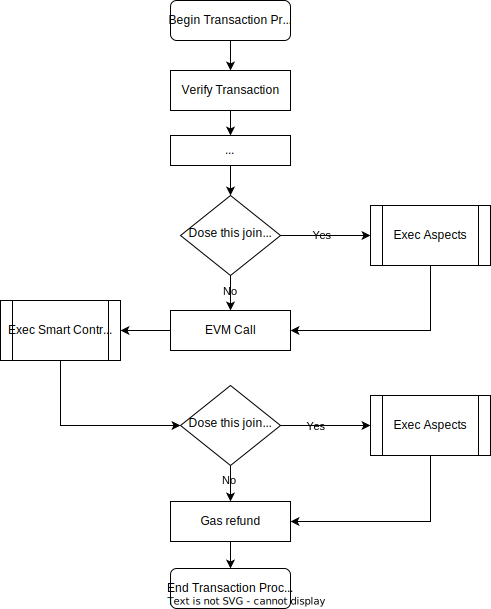
\includegraphics[width=0.5\textwidth]{sections/join-point-model-overview.png}
  \caption{Join Point Model}
\end{figure}

To provide a clearer understanding of how Aspect Programming works, let's walk through the transaction processes using an example. In this scenario, there is a smart contract with a vault function and a large deposit. The goal is to protect this smart contract at runtime to avoid illicit attacks that might illegally move out deposits. For this purpose, an Aspect is designed to be responsible for monitoring and verifying any deposit changes in the vault after smart contract execution. If there is an unexpected fund flow, the Aspect will revert the suspicious transaction. The Aspect execution is triggered after the smart contract execution when a transaction calls the smart contract.

\subsection{Aspect and Join Points}
An Aspect is implemented as a class that extends the Aspect base class. It contains methods that represent join points where additional logic can be injected. Here's an example implementation of an Aspect:

\begin{verbatim}
class SecurityAspect extends Aspect {
  @joinpoint
  postTxExecute(jpCtx: JPContext) {
    if (jpCtx.currentCall().methodName() == "withdraw") {
      let mintAmount = jpCtx.currentCall().params()[1];
      let actualVaultEtherFlow = jpCtx.stateChange(jpCtx.tx.to()).ether().diff();
      
      if (mintAmount != actualVaultEtherFlow) {
        jpCtx.txControl().revert();
      }
    }
  }
}
\end{verbatim}

In this example, the \texttt{postTxExecute} method serves as an entry point for the join point, which is triggered once the Ethereum Virtual Machine (EVM) completes transaction execution. The method is decorated with the \texttt{@joinpoint} annotation to indicate that it should be registered as a join point.

The \texttt{JPContext} object represents the runtime context and provides information about the original transaction, transaction runtime details at the current process point, and APIs for controlling transaction behavior. It is passed as a parameter to the join point method, enabling interaction with the transaction.

The example Aspect checks if the \texttt{withdraw} function of the smart contract is invoked during transaction execution. If so, it retrieves the expected minting amount from the transaction parameters and the actual funds flow of the vault from the runtime context. If there is a discrepancy between the expected and actual amounts, indicating a potential coding error or a cyberattack, the Aspect triggers the \texttt{revert()} function provided by the transaction management object in the runtime context, resulting in the reversal of the transaction.

\subsection{Deployment and Binding}
To deploy an Aspect onto the blockchain, its bytecode is included in a deployment transaction. This transaction calls an Aspect system contract, which stores the Aspect's bytecode within the blockchain's world state. Validators within the blockchain gain access to this bytecode, allowing them to execute the Aspect's logic when triggered.

However, an Aspect is only executed when it is bound to a specific smart contract. The binding process involves the smart contract owner signing a binding transaction using their externally owned account (EOA), the same account used for deploying the smart contract. This binding transaction includes the smart contract address and the Aspect ID. When this binding transaction is executed, it triggers the Aspect system contract, establishing the binding relationship between the smart contract and the Aspect within the blockchain's world state. Only the smart contract owner has the authority to bind Aspects to their smart contract, preventing unauthorized binding attempts by other EOAs.

Once the deployment and binding transactions are successfully processed, the Aspect is deployed onto the blockchain and bound to the smart contract. This integration enhances the capabilities and security of the smart contract by incorporating the Aspect's functionality.

\subsection{Execution with Aspect}
When a transaction is initiated on a smart contract, the Aspect Programming framework runtime is activated. As the transaction begins execution, the Aspect runtime evaluates each join point to determine if there are any bound Aspects associated with the invoked smart contract. If an Aspect is bound to a join point, it is triggered upon the completion of the transaction execution.

To execute an Aspect, the Aspect runtime retrieves its bytecode from the blockchain's world state and loads it into a WebAssembly (Wasm) runtime environment. A context object is then constructed, providing relevant information about the transaction and the execution environment. Finally, the Aspect runtime invokes the entry function of the Aspect, triggering the execution of the Aspect's logic.

For example, suppose the smart contract's \texttt{withdraw} function contains logic that ensures the transferred funds always exceed the amount specified in the function parameter. If an Aspect is bound to the \texttt{postTxExecute} join point, it will be triggered at the completion of the transaction execution. The Aspect runtime retrieves the Aspect's bytecode, loads it into the Wasm runtime, constructs a context object, and invokes the Aspect's entry function. If the Aspect identifies a discrepancy between the expected and actual funds transfer, it can set a revert flag via the join point context. Upon detecting this flag, the Aspect runtime reverses the transaction, labels the result as a failure, and provides a rationale specifying that the transaction was overturned by the bound Aspect.

\subsection{Conclusion}
The Aspect Programming framework's core component is the Join Point Model (JPM), which provides hooks for injecting additional logic at specific points in the transaction and block processing flows. Aspects, which contain the additional logic, can access the runtime context and make system calls to participate in transaction lifecycle management. By binding Aspects to specific join points, smart contract owners can enhance the capabilities and security of their contracts.

In the following sections, we will delve into a detailed design of the Join Point Model and its implementation.

\section{Join Point Model}

In this section, we present the specifications, major processes, and key features of the join point model and explain how it works together with the existing blockchain paradigm\footnote{We refer to the basis of the blockchain paradigm defined in Ethereum Yellow Paper, which is a model that forms the backbone of not only Ethereum but all decentralized consensus-based transaction systems to date.} defined by Ethereum[x]. The entire formal description of JPM is laid out in Appendix A.

To better describe JPM in the context of the current blockchain paradigm, we reuse the formal notation defined in Ethereum's yellow paper[x] and extend new ones for JPM.

\subsection{The Model}

In this section, we present high-level specifications of the join point model, the detailed components are presented in the following sections.

\textbf{Aspect.} Blockchain can be viewed as a transaction-based state machine, it begins with a genesis state and incrementally execute transactions to morph it into some current state. Aspect (formally, $A$) also represents a stateful program on the blockchain. Each Aspect has its own state (formally, $\varpi$). Thus, the blockchain with Aspect encompasses two types of global states: the world states of accounts\footnote{Accounts include Externally Owned Accounts (EoA) and Contract Accounts (CA)} , (formally,  $\sigma$) and the states of Aspects, $\varpi$. 

When a transaction (formally, $T$) interacts with an Aspect, the state transition of the Aspect occurs. Formally: 

$$
\varpi_{t+1} \equiv \Gamma(\varpi_{t},T) 
$$

Here, $\Gamma$ denotes the state transition function of $A$. It allows $A$ to perform an arbitrary computation, and $\varpi$ enables $A$ to store arbitrary states between transactions. 

\textbf{Join points.} Join points (formally, $J$) represent specific lifecycle stages of transactions and blocks. In the join point model, each Aspect must register itself to a specific join point. At each join point, the registered Aspects are executed. Formally, we describe the state transition function $P$ of a join point as:

$$
P(\varpi,T)\equiv\Gamma_{A_0}(\varpi,T)\oplus\Gamma_{A_1}(\varpi^{A_0},T) \oplus ... 
$$
$$
(A_0, A_1,...) \equiv \Eta(T_t, \forall b)
$$

When a transaction $T$ goes through a join point, a list of $A$ is executed sequentially. However, not all registered Aspects at the join point will be executed, only those bound with the smart contract called by this $T$. The binding relation records(formally, $b$) are registered by the smart contract owner in advance. The query function $H$ retrieves the binding list according to the target smart contract address ($T_t$) of $T$.

\textbf{Transaction State Transition.} The transaction state transition of the Ethereum blockchain paradigm is defined as:

$$
\sigma_{t+1} \equiv \Upsilon(\sigma_{t},T)
$$

Here, $\Upsilon$ represents the state transition function of the smart contract, leading to the transition of $\sigma$. 

With Aspect, a transaction $T$ will lead to the transition of both world state $\sigma$ and Aspect state $\varpi$. The new state transition function is denoted as $\Upsilon^{'}$. Formally:

$$
(\sigma_{t+1},\varpi_{t+1}) \equiv \Upsilon^{'}(\sigma_{t},\varpi_{t},T)
$$

During the lifecycle of a transaction, it traverses through multiple join points $J$. Therefore, $\Upsilon^{'}$ can be expanded as follows:

$$
\Upsilon^{'}(\varpi, \sigma,T) \equiv P_{j_{0}}(\varpi,T) \oplus P_{j_{1}}(\varpi^{J_0},T) \oplus ... \oplus \Upsilon(\sigma,T) \oplus ... \oplus P_{j_{n}}(\varpi^{j_n-1},T)
$$

Each join point state transition function $P$ is executed sequentially, and the resulting $\varpi$ generated by the previous $P$ will be used as the input of the next $P$. 

\textbf{Block State Transition.} The blockchain state transition model of the Ethereum blockchain paradigm is formally defined as:

$$
(\sigma_{t+1}) \equiv\Pi( \sigma_{t},B) \\ B \equiv (...,(T_0,T_1,T_2,...)...)
$$
$$
\Pi( \sigma,B)\equiv \Omega(B, \Upsilon(\Upsilon( \sigma,T_0),T_1)...)
$$

Here, $\Omega$  is the block-finalization state transition function (a function that rewards a nominated party); $B$ is this block, which includes a series of transactions; and $\Pi$ is the block-level state-transition function.

With Aspect, we extend the blockchain model with an additional Aspect state, $\varpi$. Formally: 

$$
(\varpi_{t+1}, \sigma_{t+1}) \equiv\Pi(\varpi_{t}, \sigma_{t},B)
$$
$$
B \equiv (...,(T_0,T_1,T2,...)...)
$$
$$
\Pi(\varpi, \sigma,B)\equiv \Omega(B, \Upsilon^{'}(\Upsilon^{'}(\varpi, \sigma,T_0),T_1)...)
$$

Here, $\Pi$ leads to the global transition of both $\sigma$ and $\varpi$. $\Omega$  not only processes the tasks like distributing validator rewards but also processes additional work introduced by $\Gamma$, such as gas fee settlement.

\subsection{Join Points}

Each join point $J$ has specific metadata consisting of an entry point for an Aspect within the transaction or block lifecycle stage, and the interoperability interfaces with the blockchain base layer. Formally: 

$$
J \equiv(J_i, E,C,\{..., \psi_m,\psi_n,... \})
$$
$$
E \equiv (E_n, E_i, E_o)
$$

The metadata includes join point id ($J_i$), entry point definition (formally, $E$), and interoperability interfaces.

\textbf{Entry Point.} Each join point $J$ has a specific entry point function interface definition, $E$, it includes a unique function name (formally, $E_n$), input params (formally, $E_i$), and output (formally, $E_o$). The Aspect requested in $J$ must implement function $E$, while function $E$ of the Aspect will be invoked to begin the execution of this Aspect.

\textbf{Interoperability Interfaces.} The interoperability interface includes the runtime context (formally, $C$) with execution semantics for read and write, and the system call (formally, $\psi$), granting Aspect access to blockchain base layer functionalities. A $J$ might provide multiple $\psi$. By leveraging these interoperability interfaces, Aspects can modify or enhance the behavior of the transaction or block processing flow. We will discuss the details of runtime context and system call in the upcoming sections. We will continue to introduce the details of $C$ and $\psi$ in post sections.

\subsubsection{Layout}

Within the Aspect Programming, we have defined various join points throughout the lifecycle of blocks and transactions. This approach enables Aspect developers to implement substantial customizations for dApps.

\begin{figure}[ht]
  \centering
  \includegraphics[width=0.4\linewidth]{sections/join-point-layout.png}
  \caption{Layout of join point.}
  \label{fig:join_point_layout}
\end{figure}

Figure \ref{fig:join_point_layout}  shows a list of join points that might be implemented. The following table \ref{tab:join-points-table} lists the description of the join points in which we describe what Aspect might do in those join points. 

\begin{longtable}{p{4cm}p{10cm}} % Adjust the column widths as desired
    \caption{Description of join points and their corresponding actions.}
    \label{tab:join-points-table} % Add a label for referencing
    \\
    \toprule
    \multicolumn{1}{c}{Join Point} & \multicolumn{1}{c}{Description} \\
    \midrule
    \endfirsthead
    
    \multicolumn{2}{c}{{\tablename\ \thetable{} -- continued from previous page}} \\
    \midrule
    \multicolumn{1}{c}{Join Point} & \multicolumn{1}{c}{Description} \\
    \midrule
    \endhead
    
    \midrule
    \multicolumn{2}{c}{{Continued on next page}} \\
    \endfoot
    
    \bottomrule
    \endlastfoot
    
    on\_block\_initialize & Activated prior to the preparation of the block proposal. Automated transaction is allowed to be inserted at this point. \\[20pt]
    on\_tx\_verify & Triggered following the transaction signature verification. The Aspect can introduce a customized transaction verification process, which takes precedence over the built-in process. \\[30pt]
    pre\_tx\_execute & Triggered prior to the transaction execution. At this stage, the account state remains pristine, allowing Aspect to preload information as necessary. \\[30pt]
    pre\_contract\_call & Triggered before the execution of the cross-contract call. At this stage, the state of the callee remains unaltered, providing the Aspect with an opportunity to preload any necessary information. \\[30pt]
    post\_contract\_call & Triggered after the cross-contract call is executed. The Aspect can then inspect the post-call state of the contract and make subsequent execution decisions. \\[30pt]
    post\_tx\_execute & Activated once the transaction has been executed and the account states have been finalized. Subsequently, Aspect can conduct a comprehensive review of the final execution state. \\[30pt]
    on\_tx\_committed & Triggered after the transaction has been finalized, and the modified states induced by the transaction have already been flushed into the state database. At this stage, Aspect can conduct post-processing activities, such as initiating an asynchronous task that can be executed in a future block. \\[60pt]
    on\_block\_finalize & Triggered after a block has been finalized. It permits the Aspect to submit an asynchronous task that can be executed in a future block. \\[30pt]
    % Add more rows if needed
\end{longtable}


Notably, the join point delivers an abstract definition, permitting implementation variations across different blockchains. This adaptability caters to differences in exposed join points, permissible operations at the join point, as well as other platform-specific considerations.

\subsubsection{Context}

The runtime context $C$ provides Aspects with information on transaction and block processing, including information such as modified states of smart contracts, emitted events, and raw data fields of the transaction. Formally: 

$$
C \equiv (c_b, c_t, c_a, c_e) \\ 
c \equiv (p_1, p_2,...) \\ p \equiv (p_{k}, p_{v})
$$

The context is structured as a collection of key-value pairs (formally, $p$), and when an Aspect requests a specific key (formally, $p_k$), the node will provide the most recent corresponding value (formally, $p_v$) at that point of processing. For instance, a $p_k$ `tx.origin.nonce` represents the nonce field’s value in the original transaction. Within the same $B$, It is essential that at a given $J$ for a specific $T$, all nodes in the blockchain network return the same $p_v$ for that $p_k$. This ensures the consistency of $c$, thereby aligning with the consensus mechanism. Each join point defines a specific group of $p$ that are accessible for an Aspect run on it.

\textbf{Context subsets.} All $p$ in the $C$ can be categorized into four subsets (formally, $c$). $c_{b}$ includes static information of $B$, such as block hash, validator(s) signature, etc. $c_{t}$ includes static information and real-time execution data of $T$, such as input data, transaction receipts, and state changes during execution. $c_a$ is a subset that allows modification by Aspects. Each Aspect has its own namespace in $c_a$, and Aspect can only modify $p$ in its own namespace while it’s limited that only able to read $p$ in other Aspect’s namespace. $c_e$ includes some environment variables of the node, such as the network id, etc.

\textbf{Context lifecycle.} The lifecycle of a context, $C$, is confined within a single block. When a block begins processing, a new context object is created for each transaction within that block. This context holds transaction-specific data and helps maintain state consistency throughout transaction execution. Once the block's processing completes — that is, all transactions within that block have been executed — the context is destroyed. It's important to note that this doesn't impact the blockchain's overall state or the results of the transaction, which are stored permanently on the blockchain. The context's purpose is merely to hold transient data that aids transaction execution and maintain state consistency within the scope of a single block.

\subsubsection{System Call}

In Aspect, a system call (formally, $\psi$) triggers the execution of a certain system module (formally, $M$). An $M$ can be stateful, it can maintain its own states (formally, $\varpi_{M}$). Formally: 

$$
\varpi_{M_{t+1}}=\psi(\varpi_{M_t},\psi_i)
$$

Each $\psi$ has a specific input (formally, $\psi_i$). If an $M$ is stateful, the corresponding $\psi$ will lead the state transition of the given $M$, $\varpi_{M}$. $M$ provides abilities to interact with the base layer’s functionality. For example, a specific $J$ after EVM execution can offer a system call that allows Aspect to create a “just-in-time” transaction. This transaction will be executed at the end of the block or right after the current transaction. System calls provide an essential interface between Aspect and the node.

\textbf{System Call Categories.} System calls, based on their distinct functionality, can be categorized into several groups: transaction management, block management, information maintenance, communication, and protection.

\begin{itemize}
  \item Transaction management system calls empower Aspects to construct and schedule just-in-time transactions.
  \item Block management system calls allow Aspects to participate in the block-proposing stage.
  \item Information maintenance system calls grant access to node-related data.
  \item Communication system calls enable interaction between Aspects, smart contracts, and native modules.
  \item Protection system calls allow Aspects to enforce transaction lifecycle rules.
\end{itemize}

Apart from these categories, unique system calls may be implemented in projects such as Artela or other blockchain platforms, aligning with their specific requirements.

$\psi$ is a blocking operation implying that the Aspect execution is paused and awaits the completion of $\psi$ before proceeding. If $\psi$ involves persistent state modification during execution, it is essential to ensure consistency between transaction states and the modifications made by $\psi$. This is crucial because a transaction may be reverted, which would discard its associated modifications. Furthermore, the design of $\psi$ should prioritize thread safety to effectively manage concurrent transaction executions.

\subsection{Aspect}

In this subsection, we provide a description of the Aspect's runtime, gas protocols, state storage procedures, validation processes, governance mechanisms, and upgrade methodologies.

Aspect is a dynamic and autonomous system-level extension for the blockchain. It is triggered in a specific join point, running securely within a sandboxed environment. Much like a smart contract, an Aspect can uphold its own state and proffers a programmable ownership interface, thereby facilitating a variety of governance approaches.

Aspect can also be conceptualized as an event-driven state machine, where an event might be the introduction of a new block or transaction at their different lifecycle stages. Commencing from the genesis state, the Aspect sequentially handles those events, culminating in its present state. The state transition ability provided by the Aspect can be formally defined as:

\[
\varpi_{t+1} \equiv \Gamma(\varpi_t,T)
\]
\[
\Gamma(\varpi,T) \equiv \iota(\varpi_{_{A}},\varpi_{_{S}},C,\sigma)
\]

Here, $\Gamma$ is the state transition function of Aspect which takes two inputs: current state $\varpi$ and transaction $T$. When an Aspect is triggered by a transaction $T$, state transition will be applied to the state $\varpi$. To expand $\Gamma$ in a more detailed function, it can be denoted as $\iota$ which takes four inputs: Aspect state $\varpi_a$, system module state $\varpi_s$, runtime context $C$, and world state $\sigma$.

\subsubsection{Structure}

The structure of an Aspect includes the following fields:

\begin{itemize}
  \item \textbf{Id ($A_i$):} Unique identifier of Aspect, 20-byte byte array.
  \item \textbf{Version ($A_{v}$):} This is a scalar value, equivalent to the number of version changes for the Aspect, starting from 1.
  \item \textbf{Type:} This refers to the kind of Aspect. Currently, the 'Built-in Aspect' is the only type defined in the white paper.
  \item \textbf{Byte Code ($A_{c}$):} This field refers to both current and historical versions of the Aspect code.
  \item \textbf{Governance Accounts ($A_{ga}$):} These accounts can implement governance actions concerning the Aspect. These actions include version upgrades, property changes, and version deprecation. Supported account types include EoA (Externally Owned Account), CA (Contract Account), and AA (Account Abstraction).
  \item \textbf{Settlement Accounts ($A_{sa}$):} The Aspect is not portrayed as an account on the blockchain, hence it cannot retain any assets. However, these settlement accounts are capable of holding assets and facilitating payments on behalf of Aspect. The base layer adheres to an authorization protocol, jointly established by Aspect and the settlement account, to ensure the security of the assets held in the settlement accounts.
  \item \textbf{Join Points ($A_{j}$):} This field represents all join points registered by the Aspect. It's a list of join point id $J_i$.
  \item \textbf{Bindings ($A_{b}$):} This field represents all binding relationships between the Aspect and various smart contracts. It's a list of binding relation records $b$.
  \item \textbf{Properties ($A_{p}$):} Properties represent immutable storage at Aspect runtime. It is read-only during the execution in join points. Properties are limited to undergoing modifications through the Aspect configuration process.
  \item \textbf{Storage ($A_s$):} Storage refers to mutable storage at Aspect runtime, which can be dynamically read from and written to during the execution in join points.
\end{itemize}

The state of Aspect ($\varpi_a$) can be defined with the following equivalence:

\[
\varpi_{_A} \equiv (A_{v},A_{c},A_{ga},A_{sa},A_{j}, A_{b},A_{p},A_{s})
\]

\subsubsection{Lifecycle}

An Aspect's lifecycle typically consists of deployment, upgrade, configuration, binding, execution, and destruction.

\textbf{Deployment.} This phase only occurs once. During deployment, it is necessary to specify the registered join points $A_{j}$, governance account $A_{ga}$, settlement account $A_{sa}$, and initial properties $A_{p}$. If the governance and settlement accounts are not specified, the signed EoA and caller contract account will be established as both. The deployment will initialize the state of Aspect as the following:

\[
\varpi_{_A} \equiv
\begin{cases}
    (1,A_c,A_{ga},A_{sa},A_{j},0,A_{p},0) & \text{if } A_{sa} > 0 \lor A_{ga} > 0 \\
    (1,A_c,S(T),S(T),A_{j},0,A_{p},0) & \text{otherwise}
\end{cases}
\]

Here, $A_{c}$ is the byte code of the Aspect; $A_{p}$ is the properties that will be initialized by the deployment; $S$ is the function of address recovery, which computes the sender address from the transaction signature. If the settlement account or governance account of Aspect is specified ($A_{sa} > 0 \lor A_{ga} > 0$), the settlement account and governance account of the Aspect will be set with the input, otherwise the sender of the transaction will be set as $A_{ga}$ and $A_{sa}$.

\textbf{Upgrade.} The upgrade process for an Aspect is flexible and can be initiated at any point after its deployment, with no limit to how many times it can occur. During the upgrade, both the byte code of the Aspect and its registered join points can be modified. The new code becomes effective starting from the next block after the upgrade transaction has been processed. The upgrade process is defined as the following:

\[
\varpi_{{t+1}_A} \equiv U(\varpi_t{_{_{A_c}}},\varpi_t{_{_{A_v}}},\varpi_t{_{_{A_j}}},A_c,A_j)
\]
\[
U(\varpi{_{_{A_c}}},\varpi{_{_{A_v}}},\varpi{_{_{A_j}}},A_c,A_j) \equiv ((\varpi_{_{A_c}} \oplus A_{c}),(\varpi_{_{A_v}} + 1),(\varpi{_{_{A_j}}} \oplus A_j)) 
\]

The upgrade process is captured by the upgrade function $U$ which takes the current code store of the Aspect ($\varpi{_{_{A_c}}}$), current Aspect version $\varpi{_{_{A_v}}}$ , join points of current Aspect ($\varpi{_{_{A_j}}}$), new Aspect byte code ($A_c$), and new Aspect join points ($A_j$) as inputs. The code store $\varpi{_{_{A_c}}}$ and join point store $\varpi{_{_{A_j}}}$ maintain all versions of Aspect code and corresponding join points. During the upgrade process, $A_c$ and $A_j$ will be added to $\varpi{_{_{A_c}}}$ and $\varpi{_{_{A_j}}}$ with $\varpi{_{_{A_v}}} + 1$ as their key. It's important to note that smart contracts can bind to the same Aspect across different versions. This is why both $\varpi{_{_{A_c}}}$ and $\varpi{_{_{A_j}}}$ are designed to support multi-version storage. In this way, the system ensures backward compatibility while still allowing for necessary upgrades and modifications.

We will discuss the specifics of upgrade authority within the governance section.

\textbf{Configuration.} The configuration can be activated at any time after deployment, and there is no limit to the number of times. The configuration process facilitates updates to the governance account $A_{ga}$, the settlement account $A_{sa}$, and various properties $A_p$. However, these configuration modifications will not come into play until the subsequent block. The state transition Aspect 

\[
\varpi_{_{A_{t+1}}} \equiv \Iota(\varpi_{_{A_t}}, A_{ga},A_{sa},A_p)
\]

Where $\Iota$ is the configuration process of Aspect which takes four inputs: current state of Aspect $\varpi_a$, new governance account $A_{ga}$, new settlement account $A_{sa}$, and updated properties $A_p$.

The particulars of configuration authority will be explained in the governance section.

\textbf{Binding.} The binding process can be activated at any time after deployment, and there is no limit to the number of times. The process allows the smart contract owner to bind the smart contracts to this Aspect. It is defined as a system procedure $f(b)$, which we will explain in detail in section 4.3.

\textbf{Execution.} Execution of Aspect can be triggered in different ways. We design two ways to trigger the Aspect:

\begin{itemize}
  \item \textbf{Triggered at join points:} This term refers to the activation of Aspects by join points. During a specific stage in its lifecycle, a transaction traversing a join point automatically triggers the Aspect associated with its callee. The execution can be defined as the following equivalence:
  \[
  (\varpi_{_{A_{t+1}}},\varpi_{_{S_{t+1}}},C_{t+1}) \equiv \iota(\varpi_{_{A_{t}}},\varpi_{_{S_{t}}},C_{t}, \sigma_t)
  \]
  Where $\iota$ is the state transition function of Aspect at a certain join point, which takes four inputs: state of Aspect ($\varpi_{a}$) and system modules $\varpi_{s}$, runtime context $C$, and world state $\sigma$. It makes the state transition and produces new $\varpi_{a}$, $\varpi_{s}$, and $C$.
  
  \item \textbf{Triggered by external calls:} Aspects can also embody external interfaces that may be invoked manually by an EoA (Externally Owned Account). These interfaces allow querying the Aspect or transitioning its state. The definition of the external call can be explained as $\iota'$:
  \[
  (\varpi_{_{A_{t+1}}},\varpi_{_{S_{t+1}}}) \equiv \iota'(\varpi_{_{A_{t}}},\varpi_{_{S_{t}}},\sigma_{t})
  \]
  Different from $\iota$, $\iota'$ cannot access runtime context $C$ because it isn't in a transaction or block process flow.
\end{itemize}

\textbf{Destruction.} A particular version of an Aspect can be destroyed if there are no associated smart contracts. Similarly, an Aspect can be destroyed if none of its versions are linked to any smart contract. The process of destroying an Aspect can be formally depicted as:
\[
D(A,\varpi_{_A}) \equiv \emptyset
\]
Where $D$ is the destruction process which takes an Aspect ($A$) and its state $\varpi_{_A}$ as inputs, and $D$ will erase the state data $\varpi_{_A}$ from the state storage, making it empty ($\emptyset$).

\subsubsection{Execution environment}

The execution of Aspect must meet the following requirements: determinism, isolation, efficiency, quantifiable computation cost, and flexible cost payment.

\textbf{Determinism.} The execution of Aspects will be performed by the entire network of validators. Operations that introduce indeterminism can undermine consensus. Therefore, features that may result in uncertain outcomes, such as multithreading, I/O operations, or dynamic typing, are not supported during execution.

The above characteristic can be formally defined as the following:
\[
\Xi_{A_{v_1}}(A, \varpi, C) \equiv \Xi_{A_{v_2}}(A, \varpi, C)
\]
Where $\Xi_{A}$ represents the execution environment of Aspect, it is a code execution function. If we input the same Aspect $A$, Aspect state $\varpi$, and runtime context $C$ into $\Xi_{A}$, each validator ($v_1$ and $v_2$) will achieve the same result.

\textbf{Isolation.} The execution of Aspects must be securely isolated to prevent the compromise of blockchain availability and security. Three levels of isolation are required for Aspect execution:

\begin{itemize}
  \item \textit{Isolation among Aspects:} Executions of individual Aspects must remain isolated. During the execution of one Aspect, no other Aspect should interfere with its current state. Protection against such interference must extend to both memory and storage.
  \item \textit{Isolation between Aspect and smart contract:} Aspect's execution does not infringe on the state integrity of a smart contract and vice-versa. The runtime should utilize a separate memory stack and storage state trie from the EVM. Direct access to each other's state or memory is disallowed, all the communications between Aspect runtime and the EVM should be done by message passing through the system call residing in the blockchain extension and base layers.
  \item \textit{Isolation between Aspect and base layer modules:} The blockchain base layer's memory stack and state storage should be obscured from Aspects to guard against intrusion into the base layer's execution processes. The only way for Aspect to communicate with the base layer is through the limited host APIs provided by the built-in runtime.
\end{itemize}

\textbf{Efficiency.} The execution of Aspects refers to additional processes that are added to the smart contract transaction execution. This implies that it introduces extra overhead to the transaction processing. The execution environment should achieve as near-native speeds as possible.

\textbf{Quantifiable computation cost.} The computational resources used by a transaction need to be limited to ensure that the total processing time stays within a reasonable range. This is particularly crucial for maintaining the efficiency and robustness of the blockchain network. In the case of Aspects, the total computational cost, or "gas cost", of a transaction is calculated as the sum of the individual gas costs of each operation performed by the Aspect and the smart contract. Formally:

\[
A_{c} \equiv (... \oplus W_{m} \oplus W_{n} \oplus ...  ) \oplus (... \oplus \psi_{m} \oplus \psi_{n} \oplus ...  )
\]
\[
g_{_A} \equiv (...+g_{_{W_{m}}}+g_{_{W_n}}+...) + (...+g_{_{\psi_m}}+g_{_{\psi_n}}+....)
\]

Each operation can be either a WebAssembly instruction (denoted as $W$) or a system call (denoted as $\psi$). The bytecode of an Aspect ($A_c$) consists of a series of these instructions and system calls. The total gas cost of the Aspect ($g_{_A}$) is the summation of the individual gas costs for each of these operations.

By quantifying and limiting these computational resources, we can ensure that the time required for consensus on the blockchain network is kept within acceptable boundaries. This is crucial for maintaining the network's speed and efficiency.

\textbf{Gas limit.} The Aspect system, like the smart contract execution system on the blockchain, has a gas limit mechanism to prevent infinite or resource-consuming executions. This limit ensures that an Aspect operation won't monopolize the system's computational resources or cause processing delays. Before the execution of an Aspect, a gas limit is set. This gas limit is then deducted throughout the execution of the Aspect for each operation or computational step. If an Aspect's execution attempts to exceed the assigned gas limit, the execution is halted, and any state changes made during that execution are reverted. This mechanism maintains the overall performance and stability of the blockchain system while allowing complex and resource-intensive operations to be performed in a controlled manner.

\textbf{Flexible cost payment.} The method for gas payment is adjustable for Aspect execution. The gas fee can be set to be charged from the caller, the settlement account, or both.



\subsubsection{Governance}

The governance procedures of Aspect are defined as system procedures. Operations such as Aspect deployment, upgrades, and configuration are managed by the Aspect system module. These governance procedures engage corresponding system module APIs to modify Aspect. Procedures can be expressed formally as the following:

\[
O \in (I, U, D) \\
V(\varpi_{ga},a) \equiv
\begin{cases}
1 & \text{if } \varpi_{ga} = a \\
0 & \text{otherwise}
\end{cases} \\
G(\varpi_{ga},T) \equiv V(\varpi_{ga},S(T)) \oplus O 
\]

The modification to an Aspect's State Transition Function (STF) can only be carried out by the governance account of that Aspect. Any operation ($O$) that could affect the STF of Aspect, whether it be a configuration ($I$), upgrade ($U$), or destroy ($D$) operation, must first pass a validation function ($V$). The validation function checks the given address ($a$) against the current governance account of the Aspect ($\varpi_{ga}$), allowing the operation to proceed only if they match. This ensures that only the authorized governance account can perform operations that modify the STF of an Aspect. This validation process forms part of the governance process ($G$), which takes both the governance account and the operation transaction ($T$) as inputs.

The governor of Aspect can be an Externally Owned Account (EoA), Account Abstraction (AA), or Contract Account (CA). Aspect owners are free to select the governance model that best suits their needs. For instance, should an Aspect require self-governance via utility tokens, it can be facilitated through AA.

\subsubsection{Settlement}

When the blockchain's base layer necessitates payment from the Aspect, the amount will be deducted from the settlement account tied to the Aspect. This settlement account is established through a bidirectional authentication process:

\begin{itemize}
  \item Aspect can set the settlement account in deployment or configuration operation.
  \item An authorization process will be initiated by the Aspect system module to verify that the settlement account has authorized this Aspect for settlement binding operation.
\end{itemize}

Once this bond is conclusively formed, the underlying protocol of the Aspect can execute debits without condition. Management of the Account funds' liquidity must be handled externally, as insufficient funds could result in a failed execution. The deductions the Aspect may incur include gas fees or service fees. We allow the Aspect to determine the payment methods flexibly with settlement account(s). Additionally, certain system calls may necessitate payable actions, which will also be deducted from this account by default.

\subsubsection{Programming features}

We design efficient, secure, and extension-style programming features for Aspect and support Aspect to act as an extended role in the blockchain. Those features include:

\begin{itemize}
  \item \textbf{Native Governance:} Aspect supports native governance, which means changes to Aspect's code, properties, and so on must be accomplished through system procedures defined by Aspect itself. During programming, crucial runtime parameters of the protocol can be placed in properties, such as those requiring governance like pausing the protocol or adjusting fees. Hence, value modifications can be directly completed by initiating governance via system procedures, eliminating the need for additional governance-related coding and external audits. Only the government accounts of the Aspect have the authority to operate these system procedures. Governance accounts can be extended into rich governance architecture through methods like CA, AA, etc. 
  \item \textbf{In-memory State:} To minimize the cost of state loading during execution, developers may opt to cache specific storage states in memory, particularly when the number of read operations significantly surpasses the number of write operations. To ensure that the use of an in-memory state meets the requirements of deterministic execution, as well as providing efficiency and lower costs than the state storage, its underlying implementation still encapsulates the state storage. The intermediate layer offers functionalities resembling those of memory.
  \item \textbf{Semantic-rich Transaction:} Aspect leverages runtime context to supplement the semantics of a transaction. For instance, a cryptographic Aspect authenticates the multi-party signature within a transaction prior to an EVM call and stores the verification result in the context. During transaction execution in EVM, the smart contract is able to reference this signature verification result, thus eliminating the need for independent verification. Thereby, by Aspect Programming, we are able to design a semantic-rich transaction. Both Aspects and smart contracts can utilize these semantics in runtime contexts to facilitate message exchanges.
  \item \textbf{Context Exchange:} In Aspect, communication occurs through the exchange of context. This communication can take place between different Aspects or between an Aspect and a smart contract. One such scenario might involve a previous Aspect writing the KYC (Know Your Customer) flag into a transaction, which a subsequent Aspect can then read to determine its own actions.
\end{itemize}

\subsubsection{Context layout}

Runtime context of Aspect refers to the information that Aspect can use and transmit during its execution. Runtime context is composed of two parts: join point contexts and Aspect context.

\textbf{Join point contexts.} Different join points have access to various contexts. These contexts include:

\begin{itemize}
  \item \textbf{Block Contexts:} This context, which is based on current blockchain data, is accessible at all join points. It allows for queries regarding block height, as well as calls to smart contracts, among other things.
  \item \textbf{Transaction Contexts:} This context refers to the current transaction state, and it is only available at transaction-related join points. The transaction context is composed of two major parts:
    \begin{itemize}
      \item The static part provides transaction-related data such as transaction hash, transaction sender, and so on.
      \item The information generated when processing the transaction such as signature verification result, smart contract call stack, and world state changes.
    \end{itemize}
\end{itemize}

\textbf{Aspect contexts.} Aspect context refers to an in-memory data object that can be shared among Aspects. Each Aspect has its own designated data area within the Aspect context isolated by the namespace, where only the owner Aspect has the write permissions, while others retain read-only access. Aspects can use this context to transmit messages based on a mutually agreed protocol. 

\textbf{Environment contexts.} Environment context contains the overall chain environment information, including chain id, current fork, and so on.

\subsubsection{Verification}

To ensure the integrity of Aspect execution across the network, an Aspect root will be recorded in each block. At the end of the block consensus, the validator will verify the correctness of the Aspect.

The transaction receipt ($R$) of Ethereum is composed of: the type of the transaction, $R_x$, the status code of the transaction, $R_z$, the cumulative gas used in the block containing the transaction receipt as of immediately after the transaction has happened, $R_u$, the set of logs created through the execution of the transaction, $R_l$ and the Bloom filter composed from information in those logs, $R_b$:

\[
R \equiv (R_x, R_z, R_u, R_b, R_l)
\]

Verification of the Aspect requires an additional field to be added into the transaction receipt data structure, we denoted it as $R_c$, which represents the context hash of Aspect:

\[
R_c \equiv keccak(keccak(keccak(C_{a_0}),C_{a_1})...)
\]
\[
R \equiv (R_x, R_z, R_u, R_b, R_l, R_c)
\]

\textbf{Result Validation.} Each Aspect context is preserved within an in-memory lexicographically ordered map. The context root, which represents the hash of the entire Aspect context content, is calculated with the key-value pairs in the context map and documented within the transaction receipt. This procedure facilitates a concise verification of the integrity and authenticity of the Aspect contexts. Validators can confirm the Aspect result by re-executing the Aspect and comparing the resultant hash with the $R_c$ recorded in the transaction receipt.

\subsection{Binding}

Binding is the process that establishes a connection between an Aspect and a smart contract. If a smart contract binds with an Aspect, the transaction call to the smart contract will trigger the execution of the Aspect.

\[
(...,A_m, A_n,...) \equiv \Eta(a_{sc}, \forall b)
\]
\[
b \equiv (a_{sc},A_i, A_v, A_p)
\]
\[
f_{b}(b)
\]

Here, $H$ stands for a process that loads all bound Aspects of the given smart contract account address; $b$ represents the binding relation record of Aspect and smart contract, it is composed of four major pieces of information: smart contract address ($a$), bound Aspect id ($A_i$), bound Aspect version ($A_v$), and execution priority ($A_p$); binding relationships can be established via a system procedure $f_{b}$.

\subsubsection{Binding Process}

Aspect binding can be initiated through an EoA transaction or a smart contract call. To prevent unauthorized bindings for both smart contracts and Aspects, the binding process necessitates a dual-way authorization between the Aspect and the smart contract. This is crucial as the state of each can be impacted when they are combined. If this dual-way authorization is successful, the binding relationship will be recorded. Consequently, when the smart contract is triggered either by an EoA transaction or a smart contract call, the associated Aspect will also be invoked for execution.

A binding transaction or call includes the following information:

\begin{itemize}
  \item \textbf{aspect id:} This is the ID of the Aspect to bind.
  \item \textbf{aspect version:} This represents the version of the Aspect to bind. Please note, a smart contract can only bind to one version of an Aspect at a time.
  \item \textbf{contract address:} This is the address of the smart contract which will bind the Aspect.
  \item \textbf{priority:} This determines the execution order of the Aspect when triggered by the smart contract call. Aspects bound to a smart contract will be executed in a sequence. dApp developers can orchestrate this execution order according to their specific requirements.
\end{itemize}

The binding process $f(b)$ can be defined as:

\[
f(b) \equiv X(A_i) \oplus F(A_i, A_v,a_{sc},b_p)
\]

Where $F$ is the binding process. $F$ persists the binding relationship into the Aspect state $\varpi_a$ of $A_i$ and it takes four inputs: id of the Aspect ($A_i$), version of the Aspect ($A_v$), smart contract address ($a_{sc}$), and execution priority ($b_p$).

$X$ is the authorization function implemented in the smart contract. It mandates that the binding Aspect must be authorized by the smart contract $a_{sc}$. The authorization function can be formally defined as:

\[
X(A_i) \equiv
\begin{cases}
  1 & \text{if id of A is authorized} \\
  0 & \text{otherwise}
\end{cases}
\]

The function $X$ receives the id of the Aspect ($A_i$) as an input and performs a validation check. If $A_i$ is authorized, the function will return 1, indicating that the binding operation is valid and can proceed. If $A_i$ is not authorized, the function will return 0, indicating that the binding operation is invalid and should be aborted. This authorization process $X$ adds flexibility because it allows smart contracts to define their own unique validation processes. This can be particularly beneficial in systems where different smart contracts may have different requirements and standards for what constitutes an authorized operation.

\section{Aspect-Boost}
Aspect-Boost is an initial implementation of Aspect Programming on Artela, and it is a framework for any kind of blockchain to integrate to enable Aspect Programming on it. With Aspect-Boost, blockchain can support users to develop, deploy and execute Aspect on it. To integrate Aspect-Boost, blockchain nodes need to implement the adaptors of Aspect-Boots.

\subsection{Overview}

Aspect-Boots contains the following key components to boost the process of Aspect integration with different blockchains:

\begin{figure}[h]
  \centering
  \includegraphics[width=0.4\textwidth]{sections/aspect-boost.png}
  \caption{Aspect-Boost Key Components}
\end{figure}

\begin{itemize}
  \item \textbf{Aspect Core.} The Aspect core is the management module within the Aspect framework and is primarily implemented through smart contracts. It mainly comprises protocol contracts and precompiled contracts. The Aspect core manages major lifecycle processes of Aspects, including deployment, upgrade, and binding, among others. This core module meticulously scrutinizes the ownership of the Aspect in relation to the operation initiator's address, maintains the binding relationships between Aspects and smart contracts, and handles the token settlement for Aspects.
  
  \item \textbf{JPM Controller.} The join point Model controller acts as a hub, connecting the blockchain base layer and the various components of the Aspect framework. It comes into action when specific transaction or block lifecycle stages are reached. Upon the activation of a join point, the JPM controller retrieves the relevant Aspects from the Aspect core, using the address of the smart contract that invoked the action. It then constructs an instance of the Aspect runtime (ArtWASM) to execute the Aspect. In addition, the JPM controller functions as a translator, mediating interactions between the base layer and the Aspect. When an Aspect is invoking base layer functions, the JPM controller's adaptor translates this system call into the corresponding request compatible with the blockchain platform, ensuring the successful execution of the call.
  
  \item \textbf{ArtWASM.} ArtWASM is a tailored WebAssembly (WASM) runtime specifically built for executing Aspects. Functioning as a sandbox, ArtWASM ensures the secure and efficient execution of Aspects within the blockchain environment. Its design incorporates significant optimizations, aligning it perfectly with the unique requirements of Aspect execution. ArtWASM serves as a bridge between Aspects, system modules, and the JPM controller by providing a comprehensive suite of runtime APIs. These APIs act as the conduit, enabling the necessary communication between these entities. When an Aspect initiates a system call, ArtWASM routes this call to the appropriate module, thereby facilitating seamless integration and interaction across the different components of the Aspect framework.
  
  \item \textbf{System Modules.} System modules comprise a set of system-level modules that can be seamlessly integrated with the blockchain base layer. These modules enhance the functionalities of dApps, enabling them to utilize the full potential of Aspects.
  
  \item \textbf{RPC Server.} The RPC server provides a set of interfaces that are compatible with existing blockchain platforms. These interfaces facilitate the processing of Aspect operations, ensuring interoperability between different platforms.
  
  \item \textbf{Aspect SDK.} The Aspect SDK equips developers with a set of tools to build rich dApps using Aspects. It simplifies the process of incorporating Aspects into dApps and allows for more advanced and flexible applications.
\end{itemize}

\subsection{Aspect Core}

The Aspect core operates as a precompiled system contract, crafted in native code, and acts as the critical module governing Aspect life cycles. We've chosen to implement the Aspect core as a smart contract for these primary reasons:

\begin{itemize}
  \item Simpler interaction with smart contracts and the underlying world state: The Aspect core's nature as a smart contract simplifies processes such as binding authorization checks. For instance, invoking the validation interface of the smart contract is a mandatory step, which is made more straightforward by treating Aspect core as a smart contract.
  \item Compatibility with existing transaction data structure: Implementing Aspect core as a smart contract eliminates the need to create new types of transactions specifically for Aspect management. This ensures the interfaces are completely compatible with the current ones, providing seamless integration.
\end{itemize}

\textbf{Aspect Management.} The Aspect core oversees changes to the state that influence the state transition function of an Aspect. When executing such operations like deploy, upgrade, or destroy, It meticulously checks the ownership of the Aspect, validating the address of the operation initiator against that of the Aspect's governor. Only the governor of the Aspect is permitted to modify the behavior of the Aspect's state transition functions.

The Aspect core meticulously manages alterations to the state that affect an Aspect's state transition function. It performs a careful assessment of the Aspect's ownership, cross-verifying the address of the operation initiator with the address of the Aspect's governor. It's critical to understand that only the governor of the Aspect has the authority to make modifications to the behavior of the Aspect's state transition functions.

\textbf{Binding Relationship Management.} The binding relationships between Aspects and smart contracts are stored within the state of the Aspect core. Any changes to these binding relationships are reflected in the state of the Aspect core. When the blockchain receives a transaction, the Aspect core identifies the Aspects associated with the recipient's address (provided the recipient is a smart contract) and initiates the execution of the relevant join points.

\textbf{Fee Settlement.} Aspects, not being typical blockchain account objects, require a settlement account to handle token transactions. The Aspect core manages this process, as Aspects can't directly modify the balance of the settlement account. The settlement account sets an allowance amount of tokens for a given Aspect's fee settlements, and the Aspect core ensures that fees are deducted only if there is sufficient allowance.

\subsection{ArtWASM}

ArtWASM is a secure and deterministic WASM Runtime implementation and it is designed for executing Aspect. It adheres to the design of the WASM Virtual Machine - a stack-based virtual machine constructed to execute WASM binary code.

\textbf{Gas metering.} Similar to a smart contract, gas metering has been implemented in ArtWASM to quantify resource usage by Aspect. This section will outline the implementation of gas metering in the WASM environment, drawing parallels with the gas metering models used in EVM and other blockchain execution environments.

We implemented gas metering in WASM via byte code instrumentation. This involves inserting additional instructions into the WASM code to monitor and control gas consumption.

Each WASM operation can be assigned a gas cost reflecting its complexity or the resources it uses. During the instrumentation process, additional WASM instructions are inserted before each operation to deduct the operation's gas cost from the total gas available. If the operation's gas cost exceeds the remaining gas, execution is halted, preventing excessive resource usage.

Consider a simple WASM function that adds two integers. In raw WASM, this might be represented by a sequence of instructions that load the integers from memory, perform the addition, and store the result back in memory.

To instrument this function with gas metering, additional instructions would be inserted before each operation. These instructions would deduct the gas cost of the operation from the total gas available. For example, if loading an integer from memory has a gas cost of 1, and performing an addition has a gas cost of 2, the instrumented WASM code would deduct these amounts from the total gas before performing the operations.

Instrumenting gas rules in WASM can bring a new level of resource management to the platform, drawing on principles similar to those used in Move and other blockchain platforms. While the specifics would need to be tailored to the WASM environment and the specific needs of its users, the underlying concept of gas as a means of metering resource usage is a powerful one that could greatly enhance the capabilities of the WASM platform.

\textbf{Gas rule for Aspect.} The gas model of eWASM is our main reference for ArtWASM. Endowed with an extensive selection of 64-bit Integer operations, data type alterations, and operations that are type-parametric, each operation incurs a unique gas expense to accurately mirror the computational exertion involved.

Every WASM opcode has a corresponding Intel IA-32 (x86) opcode (or a series of opcodes) assigned to it. These opcodes have a fixed cycle count, which Intel refers to as latency. This methodology uses a particular CPU model from the Sky Lake architecture (Intel Xeon Platinum 8175M, one of the most used CPUs by AWS EC2), similar to CPUs fabricated in 2018, to provide a reasonable average depiction of the Artela nodes. It is presumed that a 2.5 Ghz model embodies the average, with the clock rate approximately equaling 2,500,000,000 cycles per second. An additional supposition establishes that 1 second of CPU execution is equivalent to 10 million gas, meaning that 1 gas equals 0.1 us. This leads to 0.004 gas per cycle. Moreover, it is stipulated that the gas costs undergo regular adjustments, ideally every three years, in tandem with the consistent enhancements in CPUs and the routine upgrade of hardware for Artela nodes.

The WASM opcodes demand less computational power in contrast to EVM opcodes. EVM opcodes work on 256 bits of data, while WASM opcodes are restricted to a maximum of 64 bits. This means it takes four instructions, at the very least, to match EVM. Most arithmetic instructions in EVM cost 3 gas, translating to 0.75 gas for most 64-bit WASM instructions. This variance in processing requirements brings forth the notion of particles. Within the system, Aspect gas measurements are logged in a 64-bit variable with 4 decimal digits precision. When transitioning the WASM gas count to EVM gas, it is divided by 10,000 and rounded upwards. If the outcome is less than 0, it is then adjusted to 1.

\textbf{Runtime Pool.} During the lifecycle of a transaction or smart contract call, an instance of Aspect will be invoked multiple times. If the runtime instance is reinstantiated every time, it will bring significant delays to the execution. The following is some data we have measured:

\begin{center}
\begin{tabular}{|c|c|}
  \hline
  Method & Time Cost (micro-seconds) \\
  \hline
  NewEngine & 276 \\
  NewStore & 43 \\
  NewModule & 6395 \\
  NewLinker & 26 \\
  Function Link & 1034 \\
  \hline
\end{tabular}
\end{center}

ArtWASM's built-in runtime pool has made these overheads negligible by caching the runtime instances in an LRU cache and reusing the instances when needed.

\subsection{JPM Controller}

The JPM Controller is a pivotal component in the Aspect Boost, serving as the central hub between the blockchain base layer and Aspects. One of its main roles is providing a join point adaptor, an interface designed for integration with various blockchain platforms. This adaptor offers a set of interfaces akin to the blockchain base layer, allowing Aspects to be triggered at the appropriate stages throughout the block and transaction lifecycle.

Additionally, blockchains are required to implement a set of interfaces defined by the join point adaptor. This allows the join point controller to make system calls to the appropriate base layer modules, ensuring seamless interaction between the two layers.

The join point Controller also plays a crucial role in Aspect runtime construction, taking responsibility for the assembly of the Aspect runtime instance. It injects the appropriate runtime context and host API functions into the Aspect runtime instance based on the specifications of different join points. This guarantees the correct execution of functions within the Aspect, thereby ensuring the system's successful operation.

\subsection{System Modules}

The Scheduler is a module designed to automate transaction submissions to the current block proposal. This functionality simplifies the production of on-chain automation, like automated price feeds, thereby lessening protocol dependence on off-chain networks and enhancing dApp decentralization. The Aspect system can schedule transactions in either the current or future blocks, enabling full automation of protocols with on-chain procedures. However, it's important to note that the execution of scheduled transactions is not guaranteed. In cases where the assigned block space is full, transactions may need to be rescheduled.

\textbf{ArtEVM}

ArtEVM is an enhanced version of EVM provided in Aspect-Boost. ArtEVM is able to track all the state variable changes when a smart contract is executing, which provides an overview of account states for Aspect. In the meantime, ArtEVM can execute smart contract calls in parallel, maximizing the execution performance.

An improved version of the SOLC compiler has been implemented to actualize this feature. Additional state tracing opcode will be incorporated into the EVM bytecode using the pattern outlined below:

\begin{verbatim}
...
JOURNAL <-- Records the state before the SSTORE operation
SSTORE  <-- EVM Opcode that executes a change to the world state
JOURNAL <-- Records the state after the SSTORE operation
...
\end{verbatim}

By employing this pattern, the new instructions can systematically document state changes both preceding and following the SSTORE operation. With the help of the \texttt{journal} opcodes, the recorded state changes will save in the EVM context with the following format:

ArtEVM is capable of executing EVM smart contract calls in parallel. Traditionally, the execution of transactions in EVM is sequential due to potential data conflicts. However, ArtEVM leverages techniques including multi-version state-trie and block STM algorithm to analyze potential dependencies and conflicts between transactions, enabling them to be processed simultaneously without conflict. By grouping non-conflicting transactions together and processing them in parallel, ArtEVM can significantly increase the throughput and efficiency of smart contract execution. This parallel execution capability of ArtEVM enables it to handle a greater volume of transactions, thus boosting the scalability of the blockchain network.

ArtEVM is fully compatible with Ethereum's EVM. The state tracing feature can be toggled on or off by the compiler, providing developers with a choice: they can opt for a more cost-efficient smart contract or a more secure one.

\subsection{Aspect SDK}

The Aspect SDK is a comprehensive toolkit that empowers developers to build sophisticated, dynamic decentralized applications (dApps) using Aspects. The SDK currently provides the following tools to streamline the integration of Aspects into dApps.

\begin{itemize}
  \item \textbf{RPC Client:} This tool allows developers to manage and interact with Aspects through code snippets. Since native blockchain platforms do not directly support Aspect operations, the RPC Client provides a set of interfaces related to Aspect management, mirroring those provided by the RPC Server.
  
  \item \textbf{Aspect Tool:} This command-line tool manages the entire lifecycle of Aspect development. It assists developers from creating an Aspect project to publishing, covering every stage of the Aspect development lifecycle.
  
  \item \textbf{Aspect Lib:} This collection of WASM libraries provides the basic Aspects. It includes a variety of components such as cryptographic libraries (e.g., hashing and signature verification), utility libraries (e.g., format conversions and encoding/decoding tools), and host API libraries (enabling system calls to system modules within the Aspect framework), among others.
  
  \item \textbf{ArtSOLC:} An enhanced Solidity compiler (SOLC) version, ArtSOLC can instrument state and call stack tracing code into EVM bytecode. This makes it possible to monitor state and call stacks in Aspects, further expanding the capabilities of Aspects in the context of dApps.
\end{itemize}

\subsection{RPC Server}

The RPC Server is an essential component in the Aspect framework, providing a set of interfaces compatible with existing blockchain platforms for processing Aspect-related operations. The RPC Server is responsible for handling all Aspect-related requests, such as deploying an Aspect, binding an Aspect to a smart contract, unbinding, upgrading, and others. It translates these operations into a compatible format that can be processed by the underlying blockchain base layer.

\section{New World With Aspect}

\subsection{Aspect Enables New Application Feature}

We list some of the possible features for dApp could build by Aspect Programming. Many of these are exciting and innovative directions currently being explored in the crypto world and require enhanced programmability to facilitate their implementation. 

\begin{enumerate}
  \item \textbf{Smart Contract Runtime Protection:} The current emphasis in DeFi security revolves around safeguarding smart contracts at the code level, employing measures such as OpenZeppelin's ReentrancyGuard to mitigate the risks associated with unintended reentrancy. In addition to these white-box security solutions, the Aspect-based black-box security solution offers a complementary approach, which is designed to protect the security of the protocol according to predefined rules to verify the final execution results, regardless of the specifics of the actual transactions. Key features of this solution include real-time monitoring of on-chain asset movements, proactive risk mitigation, analysis of runtime behavior to identify vulnerabilities, and ensuring the continuity of protocols by preventing catastrophic hacks and fund losses.
  
  \item \textbf{Intent Solver On-Chain:} Intent allows users to define desired outcomes (what they want), and solvers can figure out the specific route to achieve these outcomes for the user (how to get it). However, the current blockchain architecture only allows solvers to operate off-chain. Aspect enables the implementation of on-chain intent solver, enhancing the user experience in dApp. For example, a user can express, "I want to exchange X ETH for Y USDC", instead of specifying, "I want to execute the swap function from DEX that has this and that code", the Aspect-based intent solver calculates the real-time status of the DEX on-chain and triggers relevant smart contract operations to fulfill the user's intent. It enables users to customize personalized on-chain intent processing logic freely.
  
  \item \textbf{Just-in-time (JIT) Operation:} JIT operation is widely used in various scenarios, but its flexibility and timeliness are currently limited, as it can only rely on the submission of multiple transaction bundles in the off-chain memory pool. Aspect empowers users to execute logic on-chain and combine it with smart contracts in atomic transactions during the block lifecycle. This enables on-chain JIT operation huge potentiality, such as JIT liquidation, JIT LP management, and MEV-capturing AMM. Aspect brings fast, expressive DeFi innovation within one powerful architecture.
  
  \item \textbf{Native Event-Driven Action:} Native Event-driven action allows users to subscribe to real-time specific on-chain events (including token transfers, state changes, transaction completions, etc.) to trigger another related atomic task. It leverages Aspect to extend additional atomic sub-transactions after transaction execution and before transaction committing. For example, when a master non-fungible token (NFT) is transferred in a transaction, Aspect immediately transfers its associated slave NFTs based on their predefined binding rules. Native Event-driven can also be utilized for atomic asynchronous cross-chain message notifications, maintaining consistency between on-chain and off-chain states or other blockchain states. For example, by monitoring the status of NFTs on the blockchain network and triggering real-time calls to the IPFS network when specific conditions are met, Aspect ensures the final updates of NFT metadata.
    
  \item \textbf{Fully OnChain Game:} Aspect empowers users to enhance the programmability of game equipment NFTs, providing a more versatile user experience. Users can upgrade game equipment with programmability by integrating Aspect with existing OnChain game smart contracts while preserving their current data structure and operational methods. This future-proof enhancement enables further innovation opportunities within the ecosystem. For example, Aspect enables the implementation of ERC-6551 functionality within the ERC-721 protocol, allowing users to add additional features and value to game equipment while ensuring compatibility with existing protocols.

  \item \textbf{OnChain MicroService:} Users can leverage Aspect to create public on-chain services on blockchain networks, fostering collective maintenance and governance by diverse users and organizations. The Aspect-based public on-chain service model drives the growth of the blockchain ecosystem by encouraging developer participation in shared maintenance and governance. This promotes resource sharing and collaborative innovation, adding value and unlocking possibilities within the realm of decentralized finance. Additionally, it reduces development barriers and advances the adoption and application of blockchain technology.
\end{enumerate}

\subsection{Built-in Feature Layer for Decentralized Network}

It's hard for dApp to fully leverage the potential of the underlying blockchain network, and due to its limited functionality, lots of dApp lack comprehensive on-chain features, such as runtime security protection, decentralized governance, and so on, which led to a large risk for user funds on it. The integration of additional features is crucial for dApps.

Currently, users have to build off-chain components or import third-party networks for their protocol, such as the keeper network. Those additional features operate on separate networks and cannot form atomic transactions with the on-chain program, leading to new issues such as compromised security and governance complexities.

Aspect introduces a built-in "Feature Layer" for the blockchain network without third-party networks. Aspect allows extend native capabilities of the base layer, which can be free-bound by any smart contract, such as native security protection, native keeper, native index, native automation, native Oracle, native off-chain synchronize, etc. The network with Aspect not only offers the execution environment for users but also offers an extensible feature layer for them. Users can effortlessly activate these native additional features for their protocols, eliminating the need for external networks or complex off-chain systems.

A web3 world that is so smooth in protocol development and user experience has never been closer to us. Aspect will have the opportunity to unlock more innovations on the blockchain.

\subsection{Boundless Network With Customization and Composability}

Currently, if users have the requirement to implement customization on-chain, they have to build separate networks, like app-specific blockchain or app-specific layer2. They have to lose the native composability with other protocol cause of separation and relies on distant cross-chain interoperability.

With Aspect Programming, users have the ability to achieve blockchain-native customization within a single public blockchain network. This breakthrough capability overcomes the drawbacks and limitations of smart contract dApps and app-specific chains by providing dApps with the unprecedented ability to achieve native-scale composability and system-level customization.

The real boundless network will become true, and it is both scalable and extensible. User is free to expand anything they want without being concerned about the limitation of the underlay network.

\subsection{Enable Modular Application Building}

A development experience that closely resembles cloud-native applications is highly anticipated. Users will only need to focus on business logic, and other decentralized technical features will be completed by Aspect providers for users. For example, a DeFi smart contract can improve its security by binding with a public security Aspect, which is developed by security team and provider web2-level risk control ability to guard funding security.

Building in a modular manner is an important trend, which might improve the efficiency of dApp development and accelerate mass adoption of web3. Some protocols, like Celestia, enable the modular manner of building basic blockchain networks, while Aspect Programming enables the possibility of building applications in a modular manner. Users can implement the program's major features (business logic) on smart contracts and implement additional features on Aspect (or combine existing Aspects). By weaving them together, a complete dApp is produced.

\subsection{Boosting Rollups with Aspect}

Aspect Programming framework can be integrated by all execution layers, especially rollups. 

Aspect enhances rollups by addressing challenges associated with efficiently verifying proofs on the EVM. Existing methods like Optimistic (OP) and Zero-Knowledge (ZK) rollups encounter significant limits, such as bytecode bloat and inefficient implementation of fixed pairing curves. By enabling developers to handle proof verification within Aspect, a more efficient and scalable solution is achieved. For OP rollups, the potential to establish an "evm-in-wasm" mode enhances single-round non-interactive proofs. For ZK rollups, Aspect's flexibility allows for the efficient implementation of diverse pairing curves and hashing algorithms. Aspect can boost the effectiveness and viability of rollup solutions.

\section{Conclusion}

To summarize, in order to improve the extensibility of blockchain, we are doing the following work:

\begin{itemize}
  \item Design a new programming model for blockchain to enable native extension within the blockchain.
  \item Implement a framework that aligns with this programming model.
  \item Apply it to the Artela blockchain to build a boundless network that allows developers to customize application-specific extensions for their dApps.
  \item Make the framework adaptable for integration into various blockchains to enhance their extensibility.
\end{itemize}

Next, we will focus on improving the implementation of the framework to address the real challenges in the rich-dApps ecosystem of the Artela blockchain. We will also explore public universal Aspects that dApps can reuse on the Artela blockchain. Furthermore, we will continue enhancing the generality of Aspect-Boost to enable its integration into other blockchains. In the next phase, we plan to develop a new kind of Aspect that supports heterogeneous computing and unlocks more programming models for blockchain.


\section{Miscellanea}

\subsection{Heterogeneous Aspect}

In addition to the Built-In Aspect, we are architecting a novel variant, termed as the Heterogeneous Aspect, to facilitate heterogeneous computing on the blockchain. Heterogeneous computing implies native applications cultivated based on operating systems, thus exploiting operating system resources, network requests, and an array of software utilities to construct sophisticated application logic. Presently, heterogeneous computing is primarily achieved via off-chain computations, including off-chain oracles.

This design addresses the inherent limitations of the Built-in Aspect. Operating within a virtual machine, the Built-in Aspect necessitates deterministic execution, resulting in confined resource access. On the other hand, the Heterogeneous Aspect is granted network access, enabling it to undertake demanding computational tasks. For example, running AI models, which are resource-intensive and yield non-deterministic execution results, might not be viable on virtual machines. However, these tasks are feasible within the Heterogeneous Aspect's framework.

The Heterogeneous Aspect, inherently a native application, is encapsulated within containers. This approach affords an expansion in the technological repertoire of the decentralized sphere by integrating advancements such as artificial intelligence, privacy computation, real-time computation, and decentralized storage. Heterogeneous Aspect's deployment and execution are handled within a heterogeneously architected computing network, a network that shares security in mutual accordance with the main network.

The differences between Built-in Aspects and Heterogeneous Aspects are shown in the table:

\begin{table}[htbp]
    \centering
    \begin{tabular}{|l|p{6cm}|p{6cm}|}
      \hline
      & Built-in Aspect & Heterogeneous Aspect \\
      \hline
      Consensus mechanism & Loaded and executed by main net validator nodes & Can be executed by heterogeneous computing nodes, and shares security with main net validation nodes \\
      \hline
      Execution environment & Executed in a deterministic sandbox environment & Supports interaction with external heterogeneous computing platforms and external networks \\
      \hline
      Runtime restrictions & Provides limited Runtime APIs, no IO/thread/async operation/network and other high-uncertainty operation capabilities & Native program, not limited by its execution capabilities \\
      \hline
    \end{tabular}
  \end{table}
  


\subsection{Difference Between Aspect and Off-chain Computation}

Off-chain computation refers to a model similar to Oracle, where computations occur on an off-chain consensus network. The consensus is reached off-chain on the calculated results before these are input into smart contracts for utilization.
The distinctions between Aspect and off-chain computation encompass:

\begin{itemize}
  \item \textbf{Security:} Relative to L1, the contrast between Aspect and off-chain computation parallels the differences between rollup and side-chain. While one shares security with the main network, the other assumes responsibility for its security.
  \item \textbf{Interoperability:} Both Aspect and off-chain computation exhibit interoperability with contracts on L1, similar to the interoperability seen within intra-chain contract interactions and across different chains. Aspect and contract execution occur synchronously within the same transaction, whereas off-chain computation and contracts establish a distributed transaction and are typically asynchronous.
  \item \textbf{Characteristics:} As an on-chain native program, Aspect forms part of the consensus process. It can operate within the context of the consensus execution process, such as customizing transaction data structures, validating methods, and appending additional transactions.
\end{itemize}

In conclusion, Aspect and off-chain computation can act as synergistic complements to each other, empowering both smart contracts and applications. However, due to its native extension features, Aspect possesses unique functionalities that off-chain computation cannot replicate.

\subsection{About Latency Problem}

Transactions executing both a smart contract and an Aspect may exhibit elevated latency in comparison to those executing a smart contract alone. It is critical to distinguish between the following two scenarios:

\begin{enumerate}
  \item \textbf{Embedding a specific logic in an Aspect for an existing smart contract.} In the absence of an Aspect, this particular logic could be executed within off-chain components, thus not contributing to increased on-chain latency. However, if we shift this logic from off-chain components to on-chain Aspects, the transaction latency would escalate.
  \item \textbf{Implementing specific functionality via an EVM-based smart contract augmented by a WASM-based Aspect.} Were this specific functionality to be implemented exclusively by the EVM-based smart contract, transaction calls to this functionality would exhibit increased latency, as the WASM-based Aspect executes at a faster rate than the smart contract. In this scenario, the Aspect mitigates the latency.
\end{enumerate}

Despite these two scenarios seemingly contradicting each other, it is a fallacy to assume that Aspects inherently increase latency. The latency is predominantly determined by the transaction's gas limit. Given the same latency, transactions executed through an Aspect can utilize more gas.

The Aspect functionality enables the Artela blockchain to configure higher gas limits than other EVM-compatible blockchains. To exploit Aspect's capabilities to the fullest and maximize the transaction gas limit, Artela is designed to support parallel execution of transactions.

\newpage
\section*{Appendix A}

\subsection*{1. Identifiers}
\begin{align*}
\text{World State of Accounts:} & \quad \sigma \\
\text{Aspect:} & \quad A \\
\text{World State of Aspects:} & \quad \varpi \\
\text{Transaction:} & \quad T \\
\text{Block:} & \quad B \\
\text{Smart Contract STF:} & \quad \Upsilon \\
\text{Aspect STF:} & \quad \Gamma \\
    \text{Expanded Aspect STF:} & \quad \iota \\
\text{Block-Level STF:} & \quad \Pi \\
\text{Block Finalization Function:} & \quad \Omega \\
\text{Join-Point:} & \quad J \\
\text{Join-Point STF:} & \quad P \\
\text{Join-Point Entry Point:} & \quad E \\
\text{Aspect Runtime Context:} & \quad C \\
    \text{Aspect Runtime Context Group:} & \quad c \\
    \text{Aspect Runtime Context Group Key Pair:} & \quad p \\
\text{System Call:} & \quad \psi \\
\text{System Module:} & \quad M \\
\text{Aspect Operations:} & \\
    \quad \text{Destruction:} & \quad D \\
    \quad \text{Configuration:} & \quad I \\
    \quad \text{Upgrade:} & \quad U \\
\text{Receipt:} & \quad R \\
\text{Aspect Core Process:} & \quad H \\
\text{Aspect Binding:} & \quad b \\
\text{Aspect Authorization Process:} & \quad X \\
\text{Not exist:} & \quad \varnothing \\
\text{Gas cost:} & \quad g \\
\end{align*}

\subsection*{2. Definitions}
\begin{align*}
\text{Join-Point and Join-Point Entry Point:} & \\
J & \equiv (J_i, E, C, \{ \ldots, \psi_m, \psi_n, \ldots \}) \\
E & \equiv (E_n, E_i, E_o) \\
\text{Runtime Context:} & \\
C & \equiv (c_b, c_t, c_a, c_e) \\
c & \equiv (p_1, p_2, \ldots) \\
p & \equiv (p_k, p_v) \\
\text{Aspect State:} & \\
\varpi_{_A} & \equiv (A_v, A_c, A_{ga}, A_{sa}, A_j, A_b, A_p, A_s) \\
\text{Aspect Code and Gas Cost:} & \\
A_c & \equiv (\ldots \oplus W_m \oplus W_n \oplus \ldots) \oplus (\ldots \oplus \psi_m \oplus \psi_n \oplus \ldots) \\
g_{_A} & \equiv (\ldots + g_{_{W_m}} + g_{_{W_n}} + \ldots) + (\ldots + g_{_{\psi_m}} + g_{_{\psi_n}} + \ldots) \\
\end{align*}

\subsection*{3. Evaluations}
\begin{align*}
\text{Aspect STF:} & \\
\varpi_{t+1} & \equiv \Gamma(\varpi_t, T) \\
\Gamma(\varpi, T) & \equiv \iota(\varpi_{_A}, \varpi_{_S}, C, \sigma) \\
\text{Join-Point STF:} & \\
P(\varpi, T) & \equiv \Gamma_{A_0}(\varpi, T) \oplus \Gamma_{A_1}(\varpi^{A_0}, T) \oplus \ldots \\
(A_0, A_1, \ldots) & \equiv \Eta(T_t, \forall b) \\
\text{Transaction STF:} & \\
\text{Legacy Ethereum:} & \\
\sigma_{t+1} & \equiv \Upsilon(\sigma_t, T) \\
\text{With Aspect:} & \\
(\sigma_{t+1}, \varpi_{t+1}) & \equiv \Upsilon'(\sigma_t, \varpi_t, T) \\
\Upsilon'(\varpi, \sigma, T) & \equiv P_{j_0}(\varpi, T) \oplus P_{j_1}(\varpi^{J_0}, T) \oplus \ldots \oplus \Upsilon(\sigma, T) \oplus \ldots \oplus P_{j_n}(\varpi^{j_n-1}, T) \\
\text{Block STF (JoinPoint + Smart contract):} & \\
(\sigma_{t+1}) & \equiv \Pi(\sigma_t, B) \\
B & \equiv (\ldots, (T_0, T_1, T_2, \ldots), \ldots) \\
\Pi(\sigma, B) & \equiv \Omega(B, \Upsilon(\Upsilon(\sigma, T_0), T_1), \ldots) \\
\text{System Module STF:} & \\
\varpi_{M_{t+1}} & = \psi(\varpi_{M_t}, \psi_i) \\
\text{Signature Verification Function:} & \\
a & \equiv S(T) \\
\end{align*}

\subsection*{4. Aspect Operations \& Processes}
\begin{align*}
\text{Aspect Deployment:} & \\
\varpi_{_A} & \equiv
\begin{cases}
(1, A_c, A_{ga}, A_{sa}, A_j, 0, A_p, 0) & \text{if } A_{sa} > 0 \text{ or } A_{ga} > 0 \\
(1, A_c, S(T), S(T), A_j, 0, A_p, 0) & \text{otherwise}
\end{cases} \\
\text{Aspect Upgrade:} & \\
\varpi_{{t+1}_A} & \equiv U(\varpi_{t_{_{A_c}}}, \varpi_{t_{_{A_v}}}, \varpi_{t_{_{A_j}}}, A_c, A_j) \\
U(\varpi_{_{A_c}}, \varpi_{_{A_v}}, \varpi_{_{A_j}}, A_c, A_j) & \equiv ((\varpi_{_{A_c}} \oplus A_c), (\varpi_{_{A_v}} + 1), (\varpi_{_{A_j}} \oplus A_j)) \\
\text{Aspect Configuration:} & \\
\varpi_{_{A_{t+1}}} & \equiv \Iota(\varpi_{_{A_t}}, A_{ga}, A_{sa}, A_p) \\
\text{Aspect Execution:} & \\
\text{Triggered by Join-Points:} & \\
(\varpi_{_{A_{t+1}}}, \varpi_{_{S_{t+1}}}, C_{t+1}) & \equiv \iota(\varpi_{_{A_{t}}}, \varpi_{_{S_{t}}}, C_{t}, \sigma_t) \\
\text{Triggered by External Calls:} & \\
(\varpi_{_{A_{t+1}}}, \varpi_{_{S_{t+1}}}) & \equiv \iota'(\varpi_{_{A_{t}}}, \varpi_{_{S_{t}}}, \sigma_{t}) \\
\text{Aspect Destruction:} & \\
D(A, \varpi_{_A}) & \equiv \varnothing \\
\text{Aspect Operation Governance:} & \\
O & \in (I, U, D) \\
V(\varpi_{ga}, a) & \equiv
\begin{cases}
1 & \text{if } \varpi_{ga} = a \\
0 & \text{otherwise}
\end{cases} \\
G(\varpi_{ga}, T) & \equiv V(\varpi_{ga}, S(T)) \oplus O \\
\text{Aspect Context Verification:} & \\
R_c & \equiv \text{keccak}(\text{keccak}(\text{keccak}(C_{a_0}), C_{a_1}), \ldots) \\
R & \equiv (R_x, R_z, R_u, R_b, R_l, R_c) \\
\text{Aspect Binding:} & \\
\end{align*}


\bibliographystyle{plain}
\bibliography{references}

\end{document}
